\chapter{Introduction}
\label{Introduction1} 


\section{Overview: Features and Setup}

\subsection{Features}
The mpFormulaPy distribution consists of two parts: the mpFormulaPy Library and the mpFormulaPy Toolbox.

\subsection{The mpFormulaPy Library}
The mpFormulaPy Library is a collection of numerical functions and procedures in multiprecision arithmetic. It is intended to be usable on multiple platforms (i.e. platforms supported by a recent version of Python) and is provided in the form of source code in Python. 

The following numerical types are supported:

\begin{itemize}		
  \item The conventional double (64 bit) precision binary floating point type (double in C).
  \item The mpf arbitray precision binary floating point type of the mpmath library.
  \item The mpi arbitray precision interval arithmetic binary floating point type of the mpmath library.
  \item The mpc arbitray precision complex binary floating point type of the mpmath library. 
  \item The mpci arbitray precision complex interval arithmetic binary floating point type of the mpmath library.
  \item The long arbitray precision integer type of the Python library. 
  \item The Fraction arbitray precision rational type of the Python library. 
  \item The Decimal arbitray precision decimal floating point type of the Python library. 
\end{itemize}

All of these types are available as real and complex scalars. vectors, and matrices.

\vpara
The mpFormulaPy Library is based on mpmath \cite{mpmath}, and the standard Python Library, including fractions.py and decimal.py.
	
\subsection{The mpFormulaPy Toolbox}	
The mpFormulaPy Toolbox provides a setup with the Ironpython compiler 2.7.4 for the Windows platform with multiple interfaces:

\begin{itemize}	
\item A .NET Framework 4.0 interface: arithmetic functions, operators and procedures are accessible in a familiar syntax. Both 32 bit and 64 bit versions are provided. This interface makes the numerical routines available to all languages with .NET Framework support, including VB.NET, C\#, JScript 2010, F\#, MS C++ (CLI), IronPython and Matlab.
\item A COM (Component Object Model) interface: multiprecision arithmetic functions and procedures, with arithmetic operators emulated as properties. Both 32 bit and 64 bit versions are provided. This interface makes the numerical routines available to all languages with COM support, including VBScript, JScript (Windows Script Host), Visual Basic for Applications, Visual Basic 6.0, OpenOffice  Basic, Lua, Ruby, PHP CLI, Perl, Python, R (Statistical System) and Mathematica.
%\item A Java interface (Java SDK 1.7 or later): multiprecision arithmetic functions and procedures, with arithmetic operators emulated as properties. Both 32 bit and 64 bit versions are provided. Based on jni4net \citep{Savara2011}.
%\item A SQLite interface: provides access from SQL to the numerical routines to manipulate arbitrary precisons numbers stored as strings.	Based on the System.Data.SQLite \citep{Hipp2014}.
\item A Names Pipes and Command Line interface: this is designed to make sure that the calling application and the routines in the library are executed in separate processes, greatly enhancing stability. 

\end{itemize}
	
In addition, the mpFormulaPy Toolbox offers the following features:	
	
\begin{itemize}		
\item A compact IDE for VB.NET and C\# (no need to install Visual Studio). The IDE provides a Code Editor, Windows Forms Designer, Debugger, Profiler, Unit Tester and Microsoft Visual Studio compatible project files. Based on a trimmed version of Sharp Develop  \citep{SharpDevelop2013}.
\item A Microsoft Excel (versions 2000 to 2013) interface: multiprecision arithmetic functions are provided for use in spreadsheet cells, using Excel's XLL interface. It is also possible to write user-defined functions and procedures in multiprecision arithmetic (provided as add-ins written in VB.NET or C\#), which run even if macro security is set to "disable all macros". Based on Excel-DNA \citep{vanDrimmelen2013}.	
\item Full access for VB.NET and C\# to the object model of MS Excel (including Intellisense support in the Code Editor). All Microsoft Excel versions from 2000 to 2013,  both 32 bit and 64 bit (only 2010 and 2013), are supported, and no other software (like PIAs) is needed. Based on NetOffice \citep{Lange2013}.
\item An OpenOffice Calc (versions 2.1 or later, incl. Apache OpenOffice Calc or LibreOffice Calc) interface: multiprecision arithmetic functions are provided for use in spreadsheet cells, using the OpenOffice Basic interface. It is also possible to write user-defined functions and procedures in multiprecision arithmetic (provided as add-ins written in VB.NET or C\#).	
\end{itemize}




\subsection{System Requirement}
\label{System Requirements}
This mpFormulaPy Toolbox has the following system requirement:

\begin{itemize}
  \item Microsoft Windows with Microsoft .NET Framework version 4.x (Full).
\end{itemize}


This mpFormulaPy Toolbox can take advantage of the following software:

\begin{itemize}
  \item Adobe Reader 8 or later, for use with mpFormulaPy's interactive help-system.
  \item Microsoft Office 2000 or later.
  \item OpenOffice (versions 2.1 or later), or Apache OpenOffice or LibreOffice.
\end{itemize}


\subsection{Installation}
\label{Installation}
The mpFormulaPy Library and Toolbox can be downloaded from 

\vpara
\href{http://mpFormula.github.io/Py/}{http://mpFormula.github.io/Py/}. 

\vpara
Unzip the downloaded file in a directory for which you have write-access.





\section{License}
\label{mpFormulaLicense}

The mpFormulaPy Library and Toolbox is free software. It is licensed under the GNU Lesser General Public License (LGPL), Version 3 (see appendix \ref{LGPLv3}).
The manual for the mpFormulaPy Toolbox (this document) is licensed under the GNU Free Documentation License, Version 1.3 (see appendix \ref{GNUFDL}).




\section{No Warranty}
\label{No Warranty} 

There is no warranty. See the GNU  Lesser General Public License, Version 3 (see appendix \ref{LGPLv3}) for details.


\section{Related Software}

The mpFormulaC  Library and Toolbox provides fast multiprecision routines written in C, with interfaces to CPython, R, .NET and COM. It can be downloaded from 

\href{http://mpFormula.github.io/C/}{http://mpFormula.github.io/C/}. 








\chapter{Tutorials}
\label{Tutorials} 

\section{Why multi-precision arithmetic?}
\label{Why multiprecision arithmetic}

An introduction to the problems of rounding errors and catastrophic cancellation can be found in \cite{Goldberg91whatevery}. Excellent reference texts are  \cite{Higham2002} and \cite{Higham2009}.

In the following paragraphs we will give a few examples of how widely used programs like MS Excel or Libreoffice Calc can give wrong results due to the fact that they are using double precision arithmetic and not multi-precision arithmetic

\subsection{Example 1: Sums}

Sums are often calculated exactly if all summands have an exact representation. If this is not the case, results can be unpredictable. In MS Excel, the formula

\begin{verbatim}
=SUM(10000000000,-16000000000,6000000000)
\end{verbatim}
 will give the correct result  \verb|0|, but the analogous formula
 \begin{verbatim}
=SUM(1E+40,-1.6E+40,6E+39)
 \end{verbatim}
returns \verb|1.20893E+24| instead of the correct result \verb|0|.

\subsection{Example 2: Standard Deviation}
Like sums, variances and standard deviations are often calculated exactly if all arguments have an exact representation. If this is not the case, results can again be unpredictable. In MS Excel, the formula
 \begin{verbatim}
=VAR(1E+30,1E+30,1E+30)
 \end{verbatim}
returns \verb|2.97106E+28| instead of the correct result \verb|0|, which should be the obvious results since all arguments are the same.


\subsection{Example 3: Overflow and underflow}

In many situations where the final result is representable in double precision, some of the interim results cause overflow or underflow. A popular example is the function $f(x,y) = \sqrt{x^2+y^2}$. With $x=3 \cdot 10^{300}$ and $y=4 \cdot 10^{300}$ the result $f(x,y) = 5 \cdot 10^{300}$ is representable in double precision, but the (naive) calculation will overflow.



\subsection{Example 4: Polynomials}

Consider the following example \cite{Cuyt_2001}: 

\vpara
For $a=77617$ and $b=33096$, calculate

\begin{equation}
Y = 333.75 b^6 + a^2  (11 a^2  b^2 - b^6 - 121 b^4 - 2) + 5.5  b^8 + \frac{a}{2b} 
\end{equation}

The correct result is $Y = -54767 / 66192 = -0.827396...$




\subsection{Example 5: Trigonometric Functions}

Trigonometric functions are sensitive to small perturbations. 

\vpara
In double precision and binary floating point arithmetic, the tangent of $x = 1.57079632679489$ is calculated as $\tan(x) = 1.48752 \cdot 10^{14}$, whereas the correct result is $\tan(x) = 1.51075 \cdot 10^{14}$. This amounts to an absolute error of $2.32287  \cdot 10^{12}$ and a relative error of $1.54\%$.

\vpara
There are also limits on the range of arguments, e.g. $\sin(10^{8})$ returns the value $0.931639...$ (with an relative error of $-6.22776 \cdot 10^{-13}$), whereas  $\sin(10^{9})$ returns an invalid result (the exact result is 0.545843...)





\subsection{Example 6: Logarithms and Exponential Functions}


Consider the following example \citep{Ghazi2010} : 

Determine 10 decimal digits of the constant

\begin{equation}
Y = 173746a + 94228b - 78487c, \quad \text{where } 
\end{equation}
\begin{equation}
a = \sin(10^{22}), b = \ln(17.1), c = \exp(0.42). 
\end{equation}

The expected result is $Y = -1.341818958 \cdot 10^{-12}$.





\subsection{Example 7: Linear Algebra}
%\subsubsection{Determinant}
%\lipsum[1]

\subsubsection{Linear Solver}
The following example is from \cite{Hofschuster2004}:

We want to solve the (ill-conditioned) system of linear equations $Ax = b$ with

\begin{equation}
A = \begin{pmatrix}
a_{11} & a_{12} \\
a_{21} & a_{22} 
\end{pmatrix}  = \begin{pmatrix}
64919121 & -159018721 \\
41869520.5 & -102558961 
\end{pmatrix}, b = \begin{pmatrix}
b_{1} \\
b_{2} 
\end{pmatrix}
= \begin{pmatrix}
1 \\
0
\end{pmatrix} , x = \begin{pmatrix}
x_{1} \\
x_{2} 
\end{pmatrix}
\end{equation}

The correct solution is $x_1 = 205117922$, $x_2 = 83739041$.

To solve this $2 \times 2$ system numerically we first use the well known formulas

\begin{equation}
x_1 = \frac{a_{22}}{a_{11}a_{22} - a_{12}a_{21}}, \quad x_2 = \frac{-a_{21}}{a_{11}a_{22} - a_{12}a_{21}},
\end{equation}

Calculating this directly in double precision gives the following wrong result:  

$x_1 = 102558961$, $x_2 = 41869520.5$

%Linear equation
%
%See also \cite{Hofschuster2001}.


%\subsection{Example 8: Special Functions}
%\subsubsection{Gamma and Beta Functions}
%\lipsum[1]
%
%\subsubsection{Inverse Normal Distribution Function}
%\lipsum[2]
%
%
%\subsubsection{F Distribution Function}
%\lipsum[3]
%
%
%
%\subsection{Example 9: Complex Numbers}
%\subsubsection{Trigonometric Functions}
%\lipsum[1]
%
%\subsubsection{Roots of a polynomial}
%\lipsum[2]
%
%
%\subsubsection{Linear Algebra}
%\lipsum[3]

%
%\newpage
%\section{Multiprecision arithmetic spreadsheet functions}
%\label{Using multiprecision arithmetic spreadsheet function in MS Excel}
%
%\lipsum[2-3]
%
%
%
%\newpage
%\section{Using multiprecision arithmetic in VB.NET and C\#}
%\label{Using multiprecision arithmetic in VB.NET and CSharp}
%\lipsum[2-3]




\newpage
\section{Graphics using Latex}
\label{Tutorial: GraphicsLatex}


pgfplots \citep{Feuersanger_2014} - A TeX package to draw normal and/or logarithmic plots directly in TeX in two and three dimensions with a user-friendly interface and pgfplotstable - a TeX package to round and format numerical tables. Examples in manuals and/or on web site.

\vpara
\href{http://pgfplots.net/}{http://pgfplots.net/}. 


\vpara
\href{http://pgfplots.sourceforge.net/}{http://pgfplots.sourceforge.net/}. 

\vpara
\href{http://pgfplots.sourceforge.net/gallery.html}{http://pgfplots.sourceforge.net/gallery.html}. 

\vpara
\href{https://www.sharelatex.com/learn/Pgfplots\_package}{https://www.sharelatex.com/learn/Pgfplots\_package}. 



\begin{figure}[ht]
	\centering
	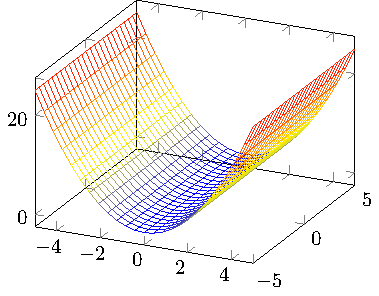
\includegraphics{figures/3Dplot.pdf}
	\caption{A pdf plot}
	\label{Fig pdf of the Distribution of the Sample Correlation Coefficient}
\end{figure}



\newpage
\section{Graphics using .NET Framework}
\label{Tutorial: Graphics}
The mpformulaPy toolbox offers a facility for producing 3D charts. The following pages give a few examples.

\begin{figure}[ht]
	\centering
	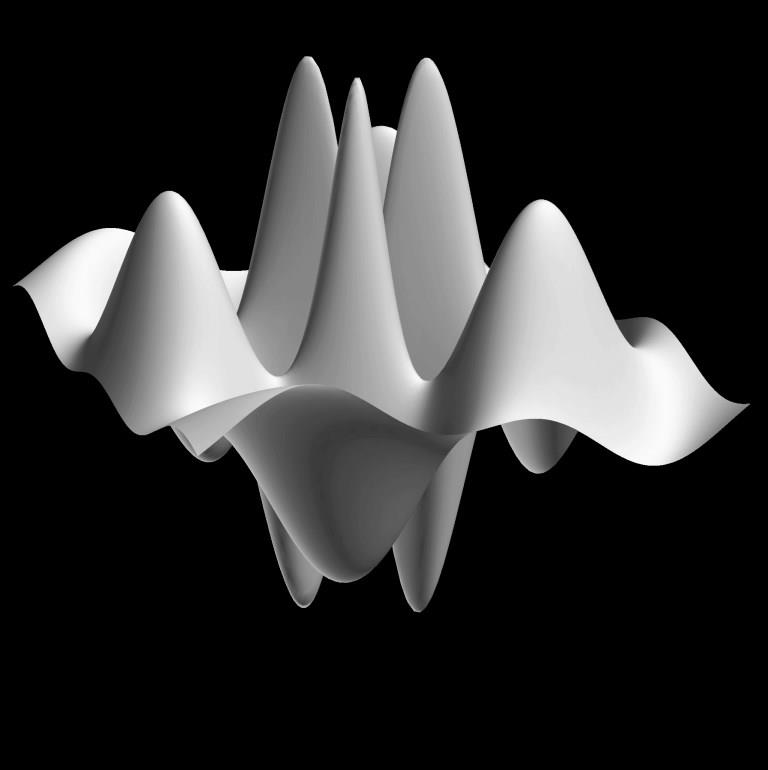
\includegraphics[scale=3.0]{Charts/jpg/SurfaceBlackAndWhite.jpg}
	\caption{plot of a 2-dimensional function}
	\label{Fig plot of a 2-dimensional function}
\end{figure}


The corresponding code is:
\lstset{language={[Sharp]C}}
\begin{lstlisting}
const double two_pi = 2 * Math.PI;
double r2 = x * x + z * z;
double r = Math.Sqrt(r2);
double theta = Math.Atan2(z, x);
result = Math.Exp(-r2) * Math.Sin(two_pi * r) * Math.Cos(3 * theta);
\end{lstlisting}


\newpage
\subsection{Surface plots for bivariate real functions}
%\lipsum[2]

The bivariate normal distribution has the following density:
\begin{equation}
	g(x,y;\rho) = \frac{1}{2 \pi \sqrt{1-\rho^2}} e^{\frac{-(x^2 -2\rho x y + y^2)}{2(1-\rho^2)}}
\end{equation}


\begin{figure}[ht]
	\centering
	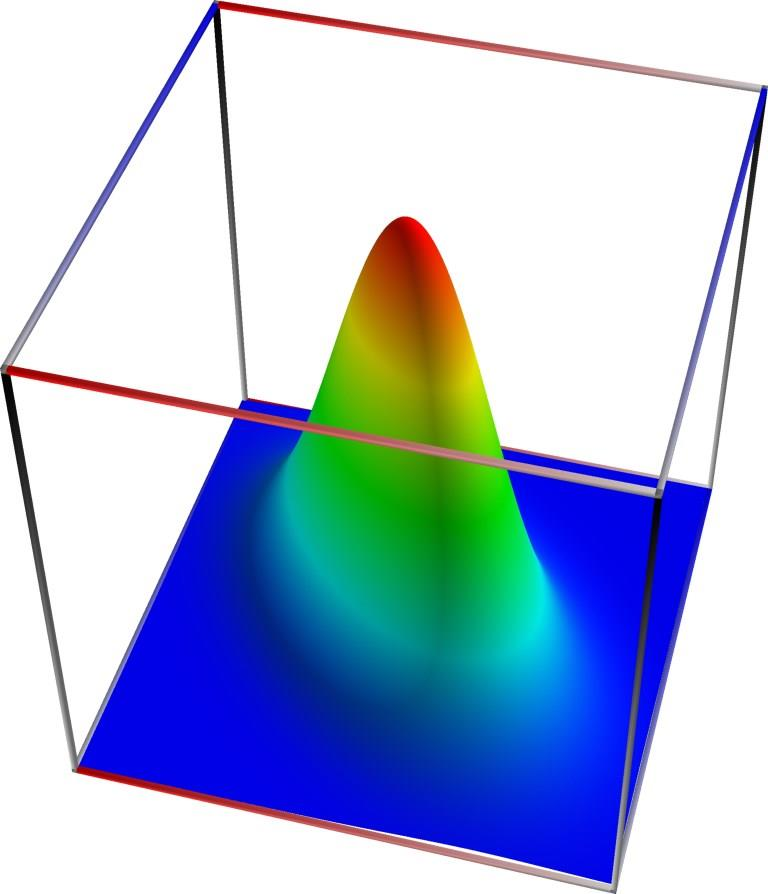
\includegraphics[scale=3.0]{Charts/jpg/BivariateNormal2.jpg}
	\caption{Surface plot of the probability density function of the bivariate normal distribution with $\rho = - 0.5$ }
	\label{Fig plot of the bivariate normal distribution}
\end{figure}


The corresponding code is:
\lstset{language={[Sharp]C}}
\begin{lstlisting}
const double two_pi = 2 * Math.PI;
double rho = -0.5;
double r2 = 1.0 - rho*rho;
double f = 1 / (two_pi * Math.Sqrt(r2));
double e = -(x*x - 2*rho*x*z + z*z)/(2*r2);
result = f * Math.Exp(e);
\end{lstlisting}


\newpage
\subsection{3D Plots of parametric functions}
%\lipsum[1]

\subsubsection{3D Plot of a Seashell}

This is a plot of a seashell. 

\begin{figure}[ht]
	\centering
	\includegraphics[scale=3.0]{Charts/jpg/Seashell.jpg}
	\caption[3D plot of a parametric function: Seashell]{3D plot of a parametric function: Seashell. umin = 0; umax = 6*Math.PI; umin = 0; umax = 6*Math.PI. Camera angles are $\theta = 135\degree$ and $\phi = -12\degree$.}
	\label{Fig 3D plot of a parametric function: Seashell}
\end{figure}


The parametrization is:
\lstset{language={[Sharp]C}}
\begin{lstlisting}
double a = Math.Exp(u / (6.0 * Math.PI));
double b = Math.Cos(v / 2.0);

x = 2.0 * (1.0 - a) * Math.Cos(u) * b * b;
z = 2.0 * (-1.0 + a) * Math.Sin(u) * b * b;
y = 1.0 - a * a - Math.Sin(v) * (1.0 - a);
\end{lstlisting}



\newpage
\subsubsection{3D Plot of Kuen's surface}

This is a plot of Kuen's surface. 

\begin{figure}[ht]
	\centering
	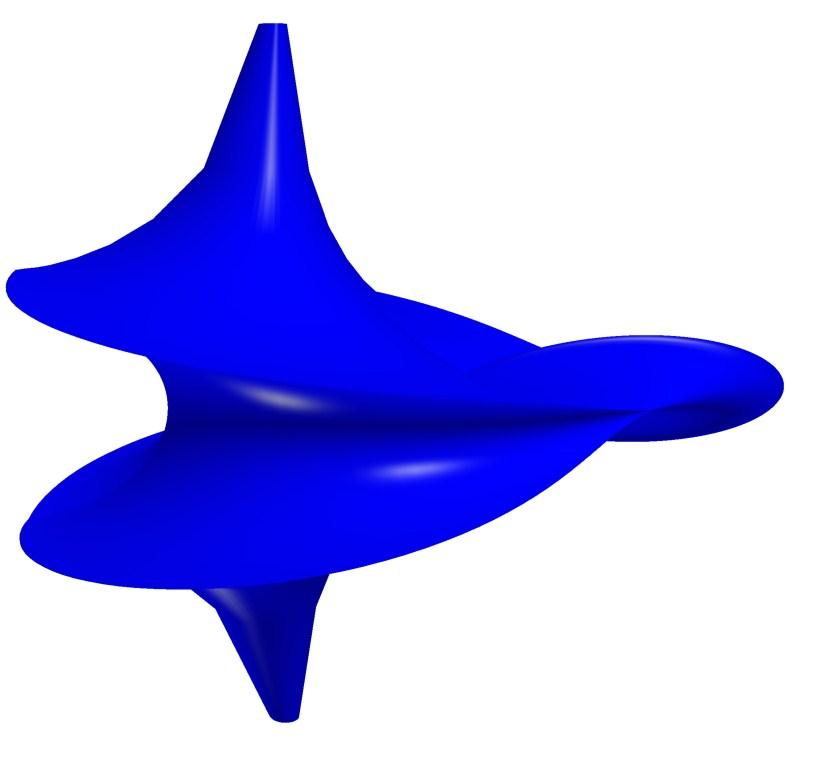
\includegraphics[scale=3.0]{Charts/jpg/KuenSurface.jpg}
	\caption[3D plot of Kuen's surface]{3D plot of a parametric function: Kuen's surface. umin = -4.5; umax = 4.5; vmin = 0.01; vmax = 3.14. Camera angles are $\theta = 135\degree$ and $\phi = -12\degree$.}
	\label{Fig 3D plot of a parametric function: Kuen's surface}
\end{figure}


The parametrization is:
\lstset{language={[Sharp]C}}
\begin{lstlisting}
double a = 1.0 * Math.Sin(v);
double b = 1.0 + u * u * a * a;

x = 2.0 * a * (Math.Cos(u) + u * Math.Sin(u)) / b;
z = 2.0 * a * (Math.Sin(u) - u * Math.Cos(u)) / b;
y = Math.Log(Math.Tan(v/2.0)) + 2.0 * Math.Cos(v) / b;
\end{lstlisting}



\newpage
\subsubsection{3D Plot of Klein's Bottle}

This is a plot of Klein's Bottle. 

\begin{figure}[ht]
	\centering
	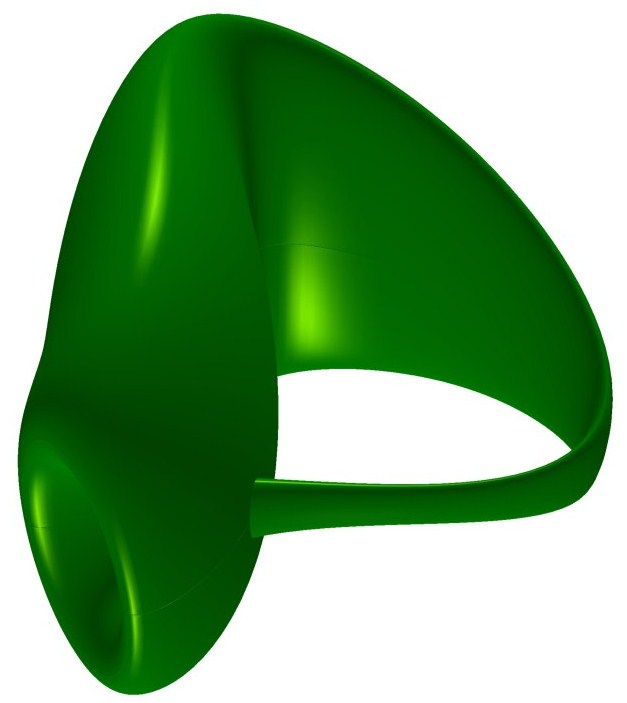
\includegraphics[scale=3.0]{Charts/jpg/KleinBottle.jpg}
	\caption[3D plot of Klein's Bottle]{3D plot of a parametric function: Klein's Bottle. umin = 0.0; umax = 3.14; vmin = 0.0; vmax = 6.28. Camera angles are $\theta = 135\degree$ and $\phi = -12\degree$.}
	\label{Fig 3D plot of a parametric function: Klein's Bottle}
\end{figure}


The following parametrization is due to Robert Israel (with some rearrangements):
\lstset{language={[Sharp]C}}
\begin{lstlisting}
double a = Math.Cos(u);
double b = Math.Sin(u);
double c = Math.Cos(v);
double a2 = a * a;
double a4 = a2 * a2;

x = -(2.0/15.0) * a * (3*c + b*(-30 + a4*(90 - 60*a2) + 5*a*c));
z = -(1.0/15.0) * b*b * (c*b* (3 - 48*a4  + 5*a*b*(1 - 16*a4)) - 60);
y = (2.0/15.0) * (3 + 5*a*b) * Math.Sin(v);
\end{lstlisting}





\newpage
\subsection{Surface plots of complex functions}
\label{Graphics: Surface plots of complex functions}
It is straight forward to produce surface plots of complex functions; these are available in two forms:

\vpara
As plots of the real and imaginary component:

\begin{figure}[ht]
	\centering
	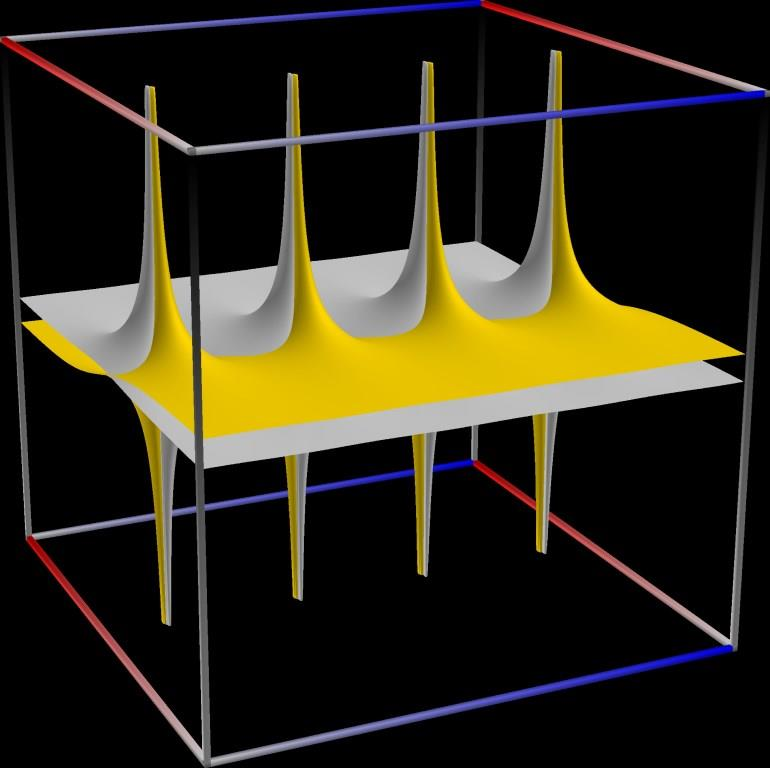
\includegraphics[scale=3.0]{Charts/jpg/ComplexSurfacePlotRealAndImaginary.jpg}
	\caption[Surface plot of the real and imaginary component of $z = \tan(x + iy)$]{Surface plot of the real ("silver") and imaginary ("gold") component of $z = \tan(x + iy)$, $-3 \leq x \leq 3$ (blue axis), $-2 \pi \leq y \leq 2\pi$ (red axis), $-10 \leq z \leq 10$ (black axis). $z$ values are truncated at $\pm 10$. There is a branch cut along the negative real axis. Camera angles are $\theta = 135\degree$ and $\phi = -12\degree$.}
	\label{Fig plot of the re and im of complex tangent}
\end{figure}



%\subsection{Pretty Formatting (specify extra digits)}

\newpage
%\subsection{File Output}
As plots of the absolute value with the phase color-coded:


\begin{figure}[ht]
	\centering
	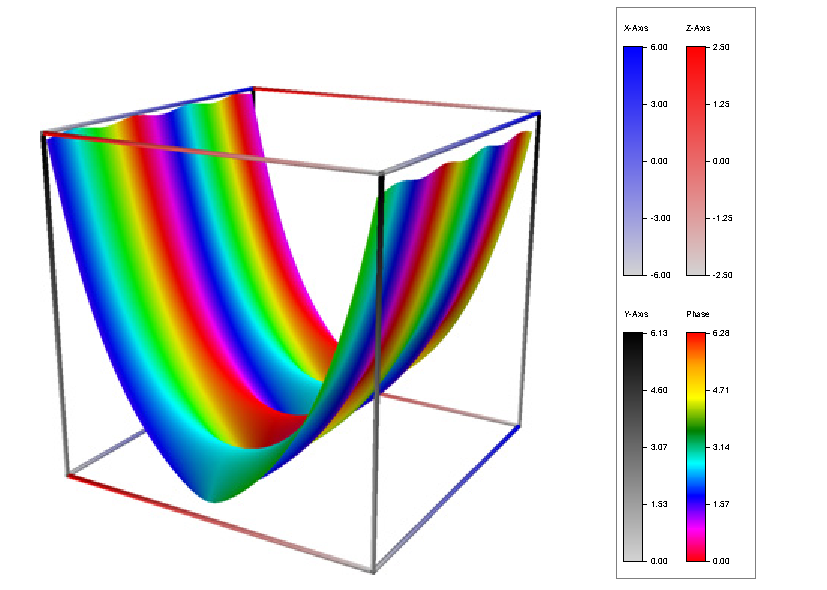
\includegraphics[scale=1.2]{Charts/pdf/SurfacePlotWithScales.pdf}
	\caption[Surface plot of the magnitude of $z = \sin(x + iy)$]{Surface plot of the magnitude and phase (color-coded) of $z = \sin(x + iy)$, $-3 \leq x \leq 3$ (blue axis), $-2 \pi \leq y \leq 2\pi$ (red axis), $-10 \leq z \leq 10$ (black axis). $z$ values are truncated at $\pm 10$. There is a branch cut along the negative real axis. Camera angles are $\theta = 135\degree$ and $\phi = -12\degree$. } 
	\label{Fig plot of the magnitude of complex sine}
\end{figure}






\newpage
\section{Eval, Options, Tables and Charts}

The following functions provide quick access to function evaluations and charts:

\vspace{0.3cm}
\begin{mpFunctionsExtract}
	\mpFunctionOne
	{Eval? String?  the result of the evaluation of an arithmetic expression, containing number and functions, but no variables.}
	{Expression? String? an arithmetic expression.}
\end{mpFunctionsExtract}


\vspace{0.3cm}
\begin{mpFunctionsExtract}
	\mpFunctionOne
	{Options? String?  an identifier for a set of calculation options.}
	{BaseOptions? String? an identifier for a set of base calculation options.}
\end{mpFunctionsExtract}


\vspace{0.3cm}
\begin{mpFunctionsExtract}
	\mpFunctionOne
	{Table? Range?  an identifier for a set of calculation options.}
	{TableRef? String? a reference for a table.}
\end{mpFunctionsExtract}


\vspace{0.3cm}
\begin{mpFunctionsExtract}
	\mpFunctionOne
	{Chart? String?  an identifier for an XML Chart.}
	{Data? Range? a reference for a data table.}
\end{mpFunctionsExtract}


